%--------------------------------------
% Spécifications du chat Felix - Camix
%
% Déploiement
%--------------------------------------

\section{Déploiement}
\label{sec:deploiement}

Le chat se compose de deux entités : les composants logiciels \textbf{Camix} et \textbf{Felix} (cf. figure~\ref{sec:deploiement:figchat}), respectivement composant serveur et client du chat.

\smallskip
Les composants Camix et Felix sont programmés en Java. Leurs exécutions nécessitent une machine virtuelle Java (ou \textit{Java Virtual Machine} - JVM) en version supérieure ou égale 8.

\smallskip
Les composants Felix et Camix communiquent via un réseau TCP/IP (\textit{Transmission Control Protocol/Internet Protocol}).

\medskip
\begin{figure}[h!]
\begin{center}
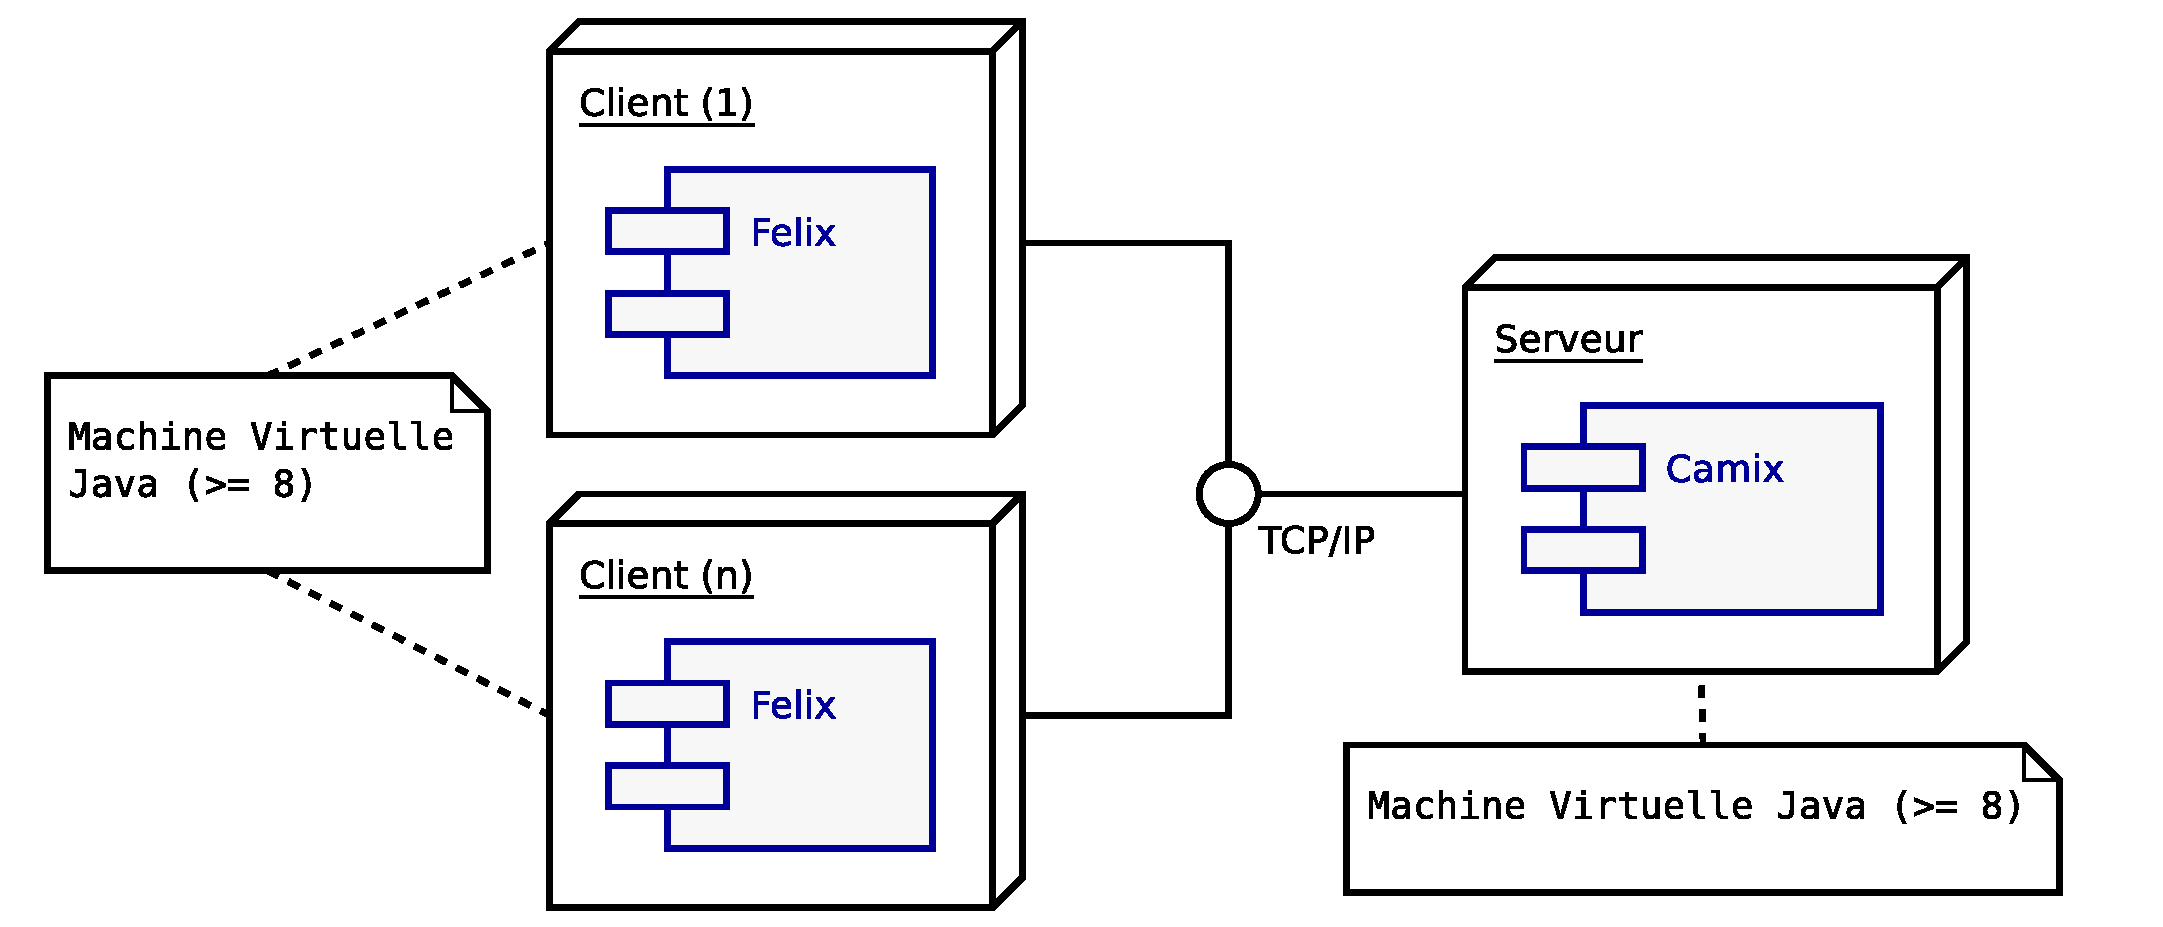
\includegraphics[width=\linewidth]{../img/Chat_Deploiement.eps}
\caption{Diagramme de déploiement du chat.}
\label{sec:deploiement:figchat}
\end{center}
\end{figure}

